\documentclass[letterpaper, 10 pt, conference]{ieeeconf}  % Comment this line out
                                                          % if you need a4paper

\IEEEoverridecommandlockouts                              % This command is only
                                                          % needed if you want to
                                                          % use the \thanks command
\overrideIEEEmargins
% See the \addtolength command later in the file to balance the column lengths
% on the last page of the document


\usepackage{graphics} % for pdf, bitmapped graphics files
\usepackage{subcaption}
\usepackage{amsmath} % assumes amsmath package installed
\usepackage{todonotes}

\title{\LARGE \bf
Roll and Pitch Motion Control for Legged Locomotion \\ on the Water Surface
}

\author{Nitish Thatte$^{1}$, Mahdi Khoramshahi$^{2}$, and Metin Sitti$^{3}$% <-this % stops a space
%\thanks{*This work was not supported by any organization}% <-this % stops a space
\thanks{$^{1}$N. Thatte is with the NanoRobotics Laboratory, Robotics Institute, Carnegie Mellon University, 5000 Forbes Ave, Pittsburgh, PA 15213, USA 
	{\tt\small nitisht at andrew.cmu.edu}}%
\thanks{$^{2}$ M. Khoramshahi is with the NanoRobotics Laboratory, Robotics Institute, Carnegie Mellon University, 5000 Forbes Ave, Pittsburgh, PA 15213, USA 
	{\tt\small khoram at andrew.cmu.edu}}
\thanks{$^{3}$ M. Sitti is the director of the NanoRobotics Laboratory, Department of Mechanical Engineering and Robotics Institute, Carnegie Mellon University, 5000 Forbes Ave, Pittsburgh, PA 15213, USA Tel: 412-268-3632
	{\tt\small sitti at cmu.edu}}
}

\begin{document}

\maketitle
\thispagestyle{empty}
\pagestyle{empty}

%%%%%%%%%%%%%%%%%%%%%%%%%%%%%%%%%%%%%%%%%%%%%%%%%%%%%%%%%%%%%%%%%%%%%%%%%%%%%%%%
\begin{abstract}
	Previous work on a biologically-inspired quadrupedal water runner robot demonstrated successful stabilization of robot pitch motions through the use of an active tail. 
This approach however, has two drawbacks: it necessitates the integration of an additional actuator and it cannot control roll motions. This paper proposes an approach for controlling the roll and height for legged robots running on the water surface. 
First, we develop a simple model for legged water surface dynamics that maps leg velocities to forces. 
We then propose an inverse dynamics control strategy based on this model that produces leg velocities that regulate the robot's height and roll angle. 
This control strategy is then applied to a detailed model of the water runner robot, and simulated experimental results are reported.

\end{abstract}

%%%%%%%%%%%%%%%%%%%%%%%%%%%%%%%%%%%%%%%%%%%%%%%%%%%%%%%%%%%%%%%%%%%%%%%%%%%%%%%%
\section{INTRODUCTION}

\section{LEGGED LOCOMOTION MODEL}
\subsection{Model Reduction}
The cited studies provide detailed and complex descriptions of generated forces and dynamics during water surface locomotion. Specifically, complexity in these models arise from the hybrid dynamics imposed by the water contact discontinuity, the nonlinearity of drag forces and the curse of dimensionality. For the purposes of controller design, the complexity of previously developed models for water surface locomotion may limit intuition, provide more information than is necessary to accomplish the desired task, and preclude the development of analytic expressions for generated force and robot state. Therefore, to simplify and focus our analysis on the dynamics required to understand the height and roll motions, we will only consider vertical dynamics produced by a simplified foot trajectory in the following analysis. 

Figure~\ref{fig:trajrob} shows the foot trajectory  and the corresponding phase portrait of the previously built water runner robot~\cite{park2010roll}. In contrast, figure~\ref{fig:trajsimp} shows a simplified circular foot trajectory and its corresponding phase diagram. We can see from the phase diagrams of the two trajectories that, especially during the plunge and stroke stages, the $y$-kinematics of the simplified foot trajectory and the actual foot trajectory are quite similar. This suggests that the $y$-dynamics produced by these two trajectories may also be similar.

\begin{figure*}[tb]
	\centering
	\begin{subfigure}[t]{0.49\textwidth}
		\centering
		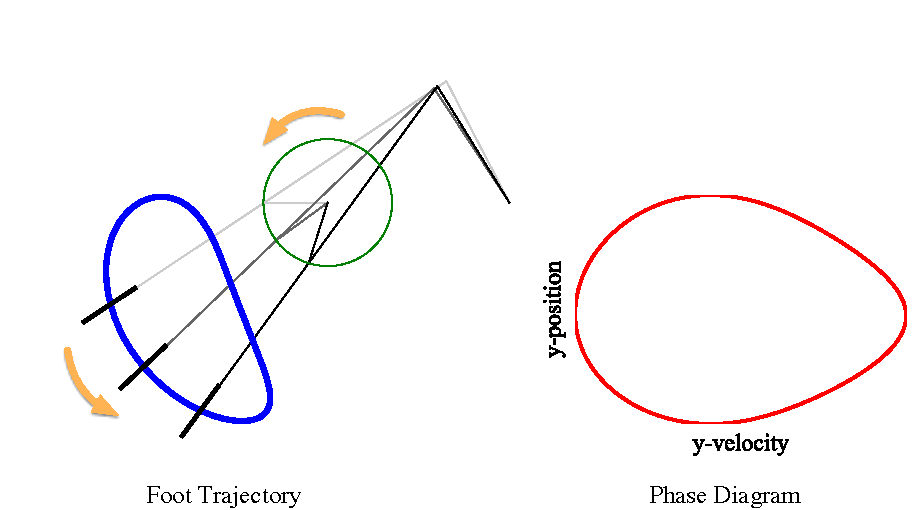
\includegraphics[width = \textwidth]{figures/foot_trajs.pdf}
		\caption{The water runner robot's foot locus in blue, with three instantaneous configurations of the leg's four-bar mechanism shown in grey. The circular path traced by the joint at the end of the input link is traced in green. In red is the phase diagram of this legged system.}
		\label{fig:trajrob}
	\end{subfigure}
    \begin{subfigure}[t]{0.49\textwidth}
		\centering
		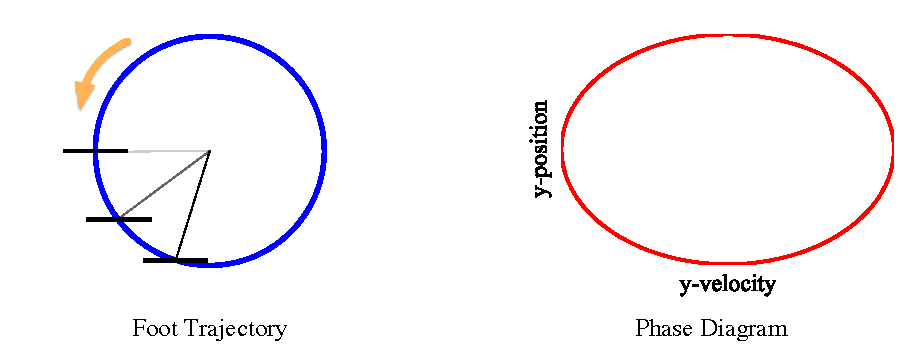
\includegraphics[width = \textwidth]{figures/foot_trajs2.pdf}
		\caption{A simplified circular foot locus in blue, with three instantaneous leg configurations shown in grey. In red is the phase diagram of this model.}
		\label{fig:trajsimp}
	\end{subfigure}
	\caption{Trajectories and phase portraits for the water runner robot and a simplified model. Note that the orientation of the foot pad of the actual robot follows the orientation of the leg, whereas the orientation of the foot pad in the simplified mode is constant.}
	\label{fig:traj}
\end{figure*}

Because we are neglecting the horizontal kinematics of the system, the circular foot trajectory can be further simplified to a foot mounted on a prismatic joint traveling vertically. We can calculate the force generated by a foot traveling on this trajectory via the equation obtained by Galsheen and McMahon \cite{glasheen1996vertical}, which states that the time-varying forces exerted by water during vertical impact of disks follows,

\begin{equation}
	F(t) = - C_D^* \left[\frac{1}{2} S \rho \dot{y}_f(t) |\dot{y}_f(t) | + S \rho g y_f(t) \right]
	\label{eq:force_t}
\end{equation}

\noindent where $F(t)$ is the time varying drag force, $C_D^* \approx 0.703$ is the drag coefficient, $\rho$ is the density of water, $g$ is the acceleration due to gravity, $S$ is the effective circular area of the disk, and $y_f(t)$ and $\dot{y}_f(t)$ are the time-varying vertical position and velocity of the disk measured in a coordinate system where positive $y$ opposes the gravity vector. 

We can write the vertical dynamics of a one legged hopping robot as in figure~\ref{fig:trajsimp} as the following system of differential equations:

\begin{equation}
	\frac{d}{dt} \begin{bmatrix} y(t) \\ \dot{y}(t) \end{bmatrix} = \begin{bmatrix} \dot{y}(t) \\ \frac{1}{m} F(y(t),\dot{y}(t), \omega) - g \end{bmatrix} 
    \label{eq:eom}
\end{equation}

\noindent Where $y(t)$ and $\dot{y}(t)$ are the position and velocity of the robot and $\omega$ is the frequency of the leg cycle. 

In order to solve for the dynamics of the system we must reduce some of the complexity outlined earlier, First, to deal with the hybrid nature of the system, we will consider the average force generated in one leg cycle instead of the continuously varying force generated by the footpad. Next, we can deal with the curse of dimensionality by assuming that the velocity of the robot body oscillations are much less than the velocity of foot oscillations. This assumption is justified given the high operational frequency range of the robot (7 - 12 Hz), the quadratic damping of the water, and the relative masses of the robot body and the footpad. This assumption implies that the velocity of the footpad is a function of only the frequency of leg cycles, $\omega$, and does not depend on the robot velocity.

Equation~\ref{eq:force_t} shows that the magnitude of the force has a quadratic dependence on foot pad speed. Consequently, the robot should generate significantly more lift by plunging its foot into the water faster than it retracts its foot. Therefore, we can split the rotational speed of the robot into two parts, a downwards speed $\omega_1$ and an upwards speed $\omega_2$

We can now develop an expression for $F_{avg}$ given $y$, $\dot{y}$, $\omega_1$ and $\omega_2$. First we define several constants: The drag coefficient of the water impact force is $b = \frac{1}{2} C_d S \rho$, the stiffness coefficient of the water impact force is $k = C_d S \rho g$, the height of the center of the foot trajectory with respect to the water is $h$, the amplitude of the foot oscillation is $A$, and the reduction in forces during the upwards part of the trajectory due to the air cavity and folding foot designs is $\alpha$. The average force on the foot over one cycle is found by integrating equation~\ref{eq:force_t} and dividing by the total time and is,

\begin{align}
    F_{avg} &= \frac{\omega_1^2 \omega_2}{\omega_1 + \omega_2} 
                \left[ \frac{b}{2 \pi} \left( A^2 \arccos \frac{h}{A} - h \sqrt{A^2 - h^2} \right) \right] \notag \\ 
            &\quad - \frac{\alpha \omega_1 \omega^2}{\omega_1 + \omega_2} 
                \left[ \frac{b}{2 \pi} \left( A^2 \arccos \frac{h}{A} - h \sqrt{A^2 - h^2} \right) \right] \notag \\
            &\quad + \frac{\omega_2}{\omega_1 + \omega_1} 
                \left[ \frac{k}{\pi} \sqrt{A^2 - h^2} - h \arccos \frac{h}{A} \right] \notag \\
            &\quad + \frac{\alpha \omega_1}{\omega_1 + \omega_1} 
                \left[ \frac{k}{\pi} \sqrt{A^2 - h^2} - h \arccos \frac{h}{A} \right] \label{eq:eom_avg}
\end{align}

\begin{comment}
\subsection{Model Fitting}

To ensure the above model represents the actual system as well as possible, we fit the model to data using two parameters via non-linear least squares regression. The first parameter we fit is $S$, the effective area of the foot pad and the second is $A$ the amplitude of the foot oscillation. We must fit these two parameters because the simplified model does not capture the time-dependent angle and submersion of the footpad. To obtain the data to fit our model to, we record the average limit-cycle heights of a simulated one legged robot for foot cycle frequencies from 40 to 100 rad/s. Then we numerically solve for the steady state height as predicted by equation~\ref{eq:eom_avg}. I.e.\ we solve for $h$ such that $F_{avg} - mg = 0$. We found best-fit amplitude is 0.0428 m and the best-fit projected area is 0.5449 times the original area. 

Figure~\ref{fig:fitheight} shows the simulated steady-state robot height in black, and the calculated steady-state height according to equation~\ref{eq:eom_avg} using the above best-fit parameters.

\begin{figure}[htb]
	\centering
	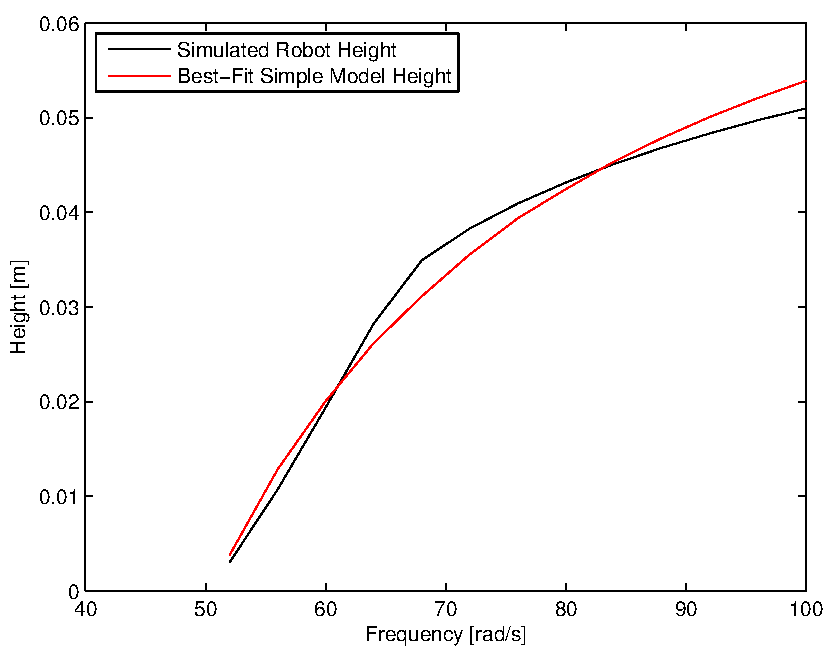
\includegraphics[width = 0.5\textwidth]{figures/fitParamsV2.pdf}
	\caption{Steady-state height of simulated robot and steady-state height calculated via equation~\ref{eq:eom_avg} using best-fit parameters Amplitude = 0.0428 m, Projected Area = 0.5449. Plotted is robot-height, which is defined as the top of the foot trajectory.} 
    \label{fig:fitheight}
\end{figure}
\end{comment}

\subsection{Four Legged Model}
To obtain a tractable model of the dynamics of a quadrupedal water runner robot, we can linearize the above equation about a nominal height and a roll angle of zero, as well as the expected leg frequency at this nominal height (obtained by solving equation~\ref{eq:eom_avg} for $\omega$ such that $F_{avg} - mg = 0$). Linearization allows us to write the force generated by one foot in the form

\begin{equation}
    F = G + A_y y + A_{\theta} \theta + B_1 \omega_1 + B_2 \omega_2
\end{equation}

\noindent Where $G$ is the state and input independent forces such as gravitational forces, $A_y y$ is the height dependent force, $A_{\theta} \theta$ is the roll angle dependent forces, and $B_{\omega_1} \omega_1$ and $B_{\omega_2} \omega_2$ are the input dependent forces.

We can then combine the linearized forces and torques produced by each leg to write the linearized dynamics of the robot in the form

\begin{equation}
    M \ddot{\vec{y}} = A \vec{y} + G + B \vec{\omega} \label{eq:rob_dyn}
\end{equation}

\noindent Where $\vec{y} = [y, \ \theta]^T$, is the output of the system and $\omega = [ \omega_1^L \ \omega_1^R \ \omega_2^L \ \omega_2^R ]^T$ is a vector of the left and right, upwards and downwards leg cycle frequencies.


\section{CONCLUSIONS}

%\addtolength{\textheight}{-12cm}   % This command serves to balance the column lengths
                                  % on the last page of the document manually. It shortens
                                  % the textheight of the last page by a suitable amount.
                                  % This command does not take effect until the next page
                                  % so it should come on the page before the last. Make
                                  % sure that you do not shorten the textheight too much.

%%%%%%%%%%%%%%%%%%%%%%%%%%%%%%%%%%%%%%%%%%%%%%%%%%%%%%%%%%%%%%%%%%%%%%%%%%%%%%%%

\section*{APPENDIX}

Appendixes should appear before the acknowledgment.

\section*{ACKNOWLEDGMENT}

This material is based upon work supported by the National Science Foundation Graduate Research Fellowship under Grant No. (NSF grant number). Any opinion, findings, and conclusions or recommendations expressed in this material are those of the authors(s) and do not necessarily reflect the views of the National Science Foundation.

\bibliographystyle{IEEEtran}
\bibliography{iros}

\end{document}
